\chapter{Evaluation, Testing \& Quality Assurance}
\label{ch:evaluation-testing}

\begin{quote}
\itshape
``If you can't measure it, you can't improve it. And if you can't improve it, you shouldn't ship it.''\\
--- Adapted from Peter Drucker
\end{quote}

\vspace{0.5cm}

\noindent
A senior engineer at a Fortune 500 company once told me: ``We spent six months building our RAG system. We spent two weeks writing tests. Guess which part broke in production?'' The answer, of course, was both---but they only \emph{noticed} the RAG failures because the tests were too shallow to catch the subtle quality regressions that had been accumulating for weeks.

Here is a truth that too many AI teams learn the hard way: \textbf{evaluation is not a phase of the development process. It is the development process.} In traditional software, you build the system first and test it after. In AI systems, you build the evaluation suite first and the system is the thing that makes the evaluations pass. This inversion is the single most important conceptual shift in this entire book.

The reason is fundamental: when you change a traditional function, you can reason about the change from the source code. When you change a prompt, swap a model, or retrain a fine-tune, you cannot reason about the change from the artifact. The \emph{only} way to know whether the change is an improvement is to measure it. If you don't have a measurement system, you are flying blind---and in production, flying blind means shipping hallucinations to customers.


\section{Evaluation as a First-Class Engineering Discipline}

In traditional software engineering, testing is a well-understood discipline with mature tooling: unit tests, integration tests, end-to-end tests, property-based tests, fuzz testing, mutation testing. Entire teams are devoted to it. No serious engineering organization would ship code without CI/CD and test coverage requirements.

LLM evaluation deserves the same status---and arguably more investment. Here is why:

\begin{itemize}[leftmargin=*]
    \item \textbf{Non-determinism}: The same input can produce different outputs on different calls. You need statistical rigor, not single-example assertions.
    \item \textbf{Subjective correctness}: ``Good enough'' depends on context, tone, audience, and use case. You need rubrics, not boolean checks.
    \item \textbf{Silent degradation}: Model updates, prompt drift, and data changes cause quality to erode gradually. You need continuous monitoring, not one-time testing.
    \item \textbf{Cascading failures}: In an agent system, a slightly worse tool-call accuracy compounds across 10 steps into a dramatically worse overall outcome. You need end-to-end evaluation, not just unit-level checks.
    \item \textbf{Adversarial risk}: Prompt injection, jailbreaking, and data poisoning are active attack vectors. You need adversarial evaluation suites alongside functional ones.
\end{itemize}

\begin{cautionbox}[The 10$\times$ Rule]
Production AI teams consistently report that evaluation infrastructure takes roughly 10$\times$ the engineering effort of the initial feature implementation. A RAG system that takes 2 weeks to build requires 20 weeks of evaluation infrastructure: golden datasets, judge prompts, regression pipelines, monitoring dashboards, and human annotation workflows. Teams that underinvest in evaluation invariably regret it within the first quarter of production operation.
\end{cautionbox}


\section{The Three-Level Evaluation Stack}

Production LLM systems require a layered evaluation approach, executed at different frequencies and costs. Figure~\ref{fig:eval-pyramid} shows the pyramid, and Figure~\ref{fig:eval-pipeline} shows how the levels connect in practice.

\begin{figure}[htbp]
\centering
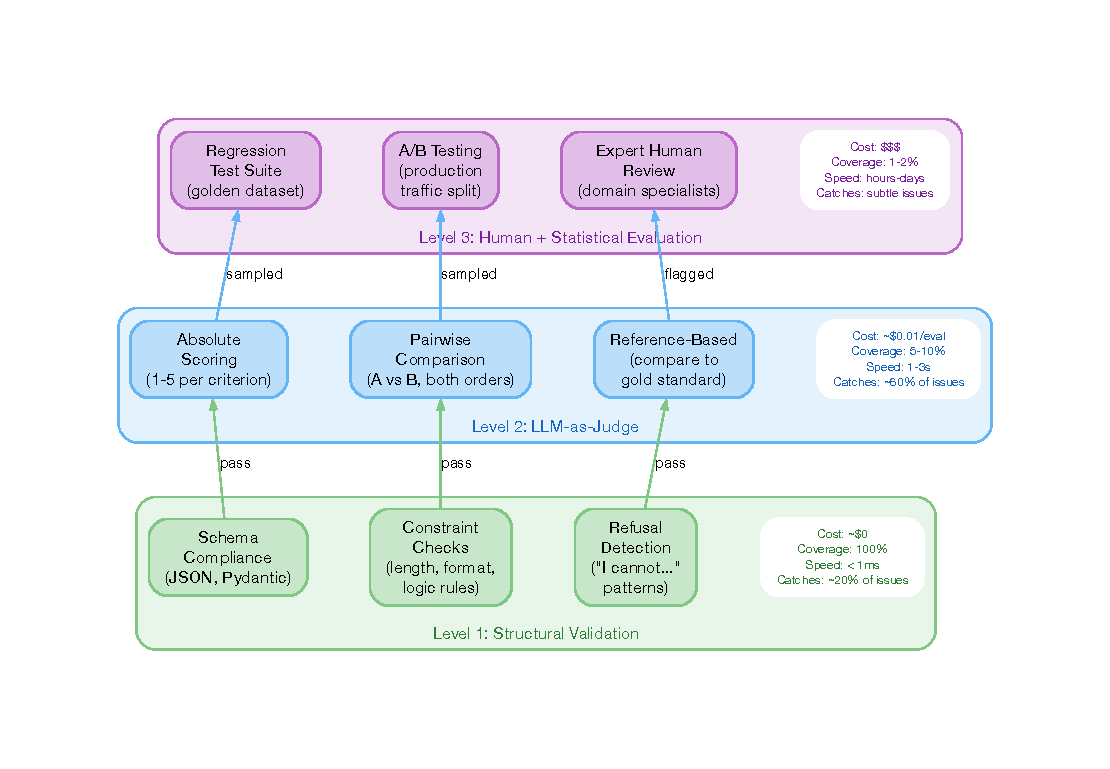
\includegraphics[width=\textwidth]{diagrams/compiled/ch08/eval-pyramid.pdf}
\caption{The AI evaluation pyramid: structural validation at the base (cheap, broad, every request), LLM-as-Judge in the middle (moderate cost, sampled), human and statistical evaluation at the top (expensive, periodic but definitive)}
\label{fig:eval-pyramid}
\end{figure}

\begin{figure}[htbp]
\centering
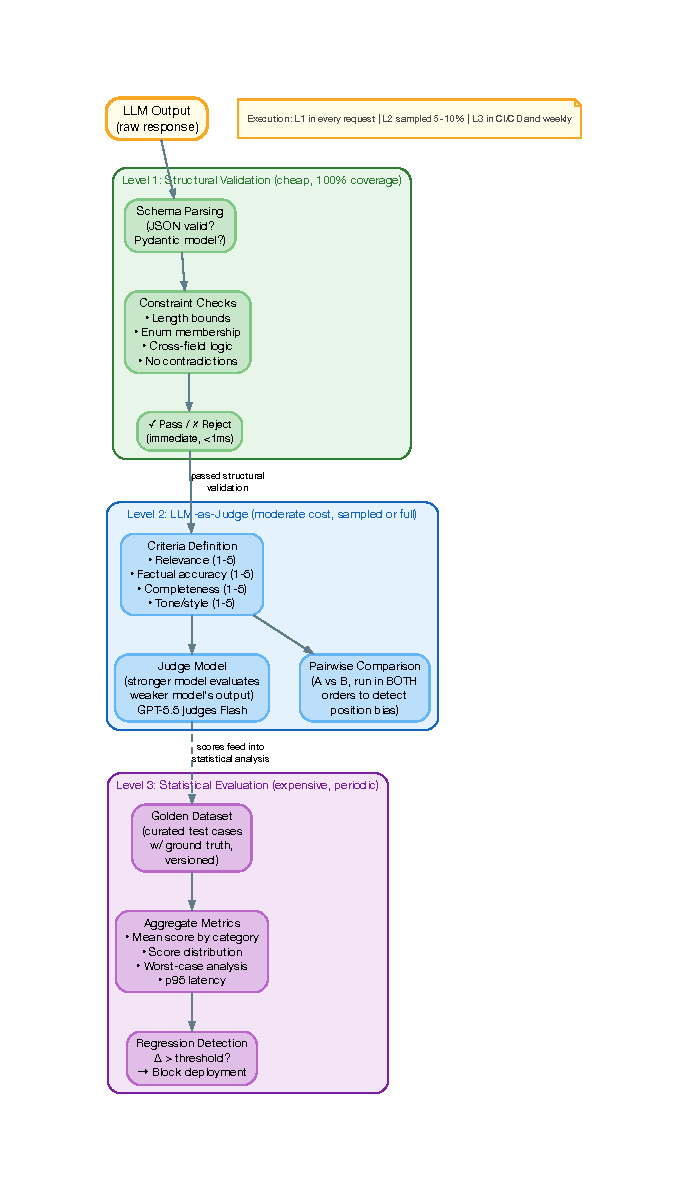
\includegraphics[width=\textwidth]{diagrams/compiled/ch08/eval-pipeline.pdf}
\caption{The three-level evaluation pipeline in practice: structural validation runs on every request ($<$1ms), LLM-as-Judge runs on a 5--10\% sample (async), statistical evaluation runs in CI/CD and weekly batches.}
\label{fig:eval-pipeline}
\end{figure}


\subsection{Level 1: Structural Validation (Every Request)}

The cheapest tests: verify that the output has the right \emph{shape}, regardless of content quality.

\begin{itemize}[leftmargin=*]
    \item \textbf{Schema compliance}: Does the JSON parse? Does it validate against the Pydantic model? Are all required fields present and correctly typed?
    \item \textbf{Constraint satisfaction}: Are enum values within defined sets? Are numbers within expected ranges? Are strings non-empty and within length bounds?
    \item \textbf{Cross-field logic}: A ``critical'' urgency with ``positive'' sentiment is contradictory. A billing issue should reference at least one product. An action summary under 10 characters is suspiciously short; over 500 suggests hallucination.
    \item \textbf{Format invariants}: Response language matches the input language. Dates are in the expected format. IDs reference entities that actually exist in your database.
\end{itemize}

Structural validation catches approximately 15--20\% of production failures at near-zero computational cost. It should be the \emph{first} check on every LLM response, gating all downstream processing. Think of it as the Validator-Corrector Proxy pattern from Chapter~\ref{ch:app-architecture}: if validation fails, retry with the error message injected into the prompt context.

\subsection{Level 2: LLM-as-Judge (Sampled)}

For content quality, use a more powerful LLM to evaluate the output. This is the practical workhorse of LLM evaluation, but it requires careful design to produce reliable signals.

\textbf{The golden rule}: The judge model should be \emph{more capable} than the model being evaluated. Use GPT-5.5 or Claude Opus 4.8 to judge Gemini 3.5 Flash outputs. Using the same model as both generator and judge introduces autoregressive confirmation bias---the Generator-Critic pattern (Chapter~\ref{ch:app-architecture}) exists precisely to avoid this.

\textbf{Judge design principles}:

\begin{enumerate}[leftmargin=*]
    \item \textbf{Separate dimensions}: Never ask a judge to produce a single ``overall quality'' score. Instead, score each dimension independently (accuracy, completeness, relevance, tone, safety) and aggregate mathematically. This prevents halo effects where a single strong dimension masks weaknesses.
    \item \textbf{Anchor the scale}: A 1--5 scale without definitions is meaningless. ``3 means adequate'' is ambiguous. ``3 means the response is factually correct but omits important context that a domain expert would include'' is actionable. Every score level needs a specific, concrete definition.
    \item \textbf{Provide reference answers}: When possible, give the judge a reference (gold-standard) answer to compare against. Judges with references produce scores that correlate 0.85+ with human evaluators; judges without references correlate around 0.65.
    \item \textbf{Use temperature 0}: Judge evaluations should be as deterministic as possible. Set temperature to 0 and use structured output to eliminate parsing variability.
\end{enumerate}

\textbf{Pairwise comparison}: Absolute scores are noisy---judges tend to be lenient. Pairwise comparison (``Is Response A or Response B better?'') is significantly more reliable. Run every comparison in \emph{both orders} (A vs B, then B vs A) to detect position bias. If the judge picks ``A'' regardless of order, A genuinely wins. If the results are inconsistent, it's a tie. Pairwise evaluation is the gold standard for model selection and A/B testing of prompts.

\textbf{Judge calibration}: Periodically compare judge scores against human annotator scores on the same 50--100 examples. Compute Spearman's rank correlation ($\rho$) and Cohen's kappa ($\kappa$). If $\rho$ drops below 0.80 or $\kappa$ drops below 0.70, the judge needs recalibration: either its prompt needs updating, or the judge model itself has drifted.

\begin{cautionbox}[Judge Bias]
LLM judges have three well-documented systematic biases: (1) \emph{verbosity bias}---they prefer longer responses even when shorter answers are more precise; (2) \emph{vocabulary bias}---they favor responses that use the same vocabulary as the evaluation prompt; (3) \emph{position bias}---they prefer whichever response appears first in a pairwise comparison. All three can be mitigated: verbosity bias through explicit rubric instructions (``penalize unnecessary elaboration''), vocabulary bias through neutral evaluation prompts, and position bias through dual-order comparison.
\end{cautionbox}


\subsection{Level 3: Statistical Evaluation on Datasets (CI/CD)}

Individual test cases can mislead. What matters is aggregate performance across a representative, versioned golden dataset.

A production golden dataset should be:

\begin{itemize}[leftmargin=*]
    \item \textbf{Curated, not random}: Hand-selected cases covering common patterns, rare edge cases, and known historical failure modes. Every case a real customer triggered.
    \item \textbf{Stratified by category}: Balanced representation of all task types. If 80\% of your cases are billing queries, you will have no signal on technical support quality.
    \item \textbf{Versioned in Git}: Changes to the golden dataset are tracked alongside prompt and model changes. You need to know: did the score drop because the model got worse, or because you added harder test cases?
    \item \textbf{Growing over time}: Every production failure becomes a new test case. Every support escalation becomes a new test case. The dataset should grow monotonically.
    \item \textbf{Sized for statistical power}: Minimum 200 cases for reliable aggregate metrics (95\% CI within $\pm$3\%). 500+ cases for per-category breakdowns with meaningful confidence intervals.
\end{itemize}

Key metrics to track: mean score by category, score \emph{distribution} (not just mean---a bimodal distribution signals systematic failure on a subset), worst-case analysis (bottom 10 cases by score), tail latency, and regression versus the locked baseline.


\section{Evaluation Metrics: From Lexical to Semantic}
\label{sec:eval-metrics}

Before diving into rubric design, it is essential to understand the landscape of evaluation metrics---how they evolved, what they measure, and where each breaks down. The history of NLP evaluation is a progression from surface-level word matching to deep semantic understanding, and each generation of metrics carries trade-offs that production teams must navigate.

\subsection{Lexical Metrics: BLEU, ROUGE, and F1}

The first generation of evaluation metrics compares \emph{words} between the model's output and a reference answer. They are fast, cheap, deterministic, and deeply flawed for evaluating modern LLM outputs.

\begin{itemize}[leftmargin=*]
    \item \textbf{BLEU} (Bilingual Evaluation Understudy): Originally designed for machine translation. Precision-oriented---it measures the degree to which words and n-grams in the generated text appear in the reference. A BLEU score penalizes outputs that use different vocabulary, even when the meaning is identical.
    \item \textbf{ROUGE} (Recall-Oriented Understudy for Gisting Evaluation): Designed for summarization evaluation. A family of metrics measuring overlap at different n-gram levels: ROUGE-1 (unigrams), ROUGE-2 (bigrams), ROUGE-L (longest common subsequence). Recall-oriented---it answers ``how much of the reference is captured?''
    \item \textbf{F1}: The harmonic mean of precision and recall, capturing both in a single score. Widely used because it is symmetric and well-understood.
\end{itemize}

\textbf{The fundamental flaw}: Lexical metrics cannot recognize semantic similarity. The sentences ``The patient responded well to the treatment'' and ``The therapy was effective for the patient'' have low lexical overlap but identical meaning. Conversely, ``The bank was steep'' and ``The bank was closed'' have high lexical overlap but entirely different meanings. For modern LLMs that generate creative, paraphrased, and contextually nuanced responses, lexical metrics systematically undercount quality.

\textbf{When lexical metrics are still useful}: Despite their limitations, lexical metrics remain valuable as \emph{fast sanity checks}: if ROUGE-L is near zero, the response is almost certainly off-topic. They also work well for highly constrained outputs (entity extraction, classification labels, structured data) where the vocabulary is fixed. Use them as Level 1 signals, not as quality arbiters.

\subsection{Semantic Metrics: Embeddings and Cross-Encoders}

The second generation uses neural models to compare \emph{meaning} rather than words.

\begin{itemize}[leftmargin=*]
    \item \textbf{BERTScore}: Computes token-level cosine similarity between the embeddings of the generated and reference texts using a pre-trained language model (typically RoBERTa). Captures synonymy and paraphrase: ``Léa is doing a great job'' and ``She's killing it'' receive high similarity despite zero lexical overlap.
    \item \textbf{Semantic Answer Similarity (SAS)}: Uses a cross-encoder model to directly score the similarity between the generated answer and the reference. Cross-encoders attend to both texts jointly, producing more nuanced similarity judgments than embedding cosine similarity.
    \item \textbf{Embedding cosine similarity}: The simplest semantic metric---embed both texts with the same model and compute cosine similarity. Fast and scalable, but less precise than cross-encoder approaches.
\end{itemize}

\textbf{The domain gap problem}: Semantic metrics are trained on general-domain text. Their performance degrades on domain-specific language (legal, medical, financial), specialized terminology, and non-English text. A BERTScore trained on Wikipedia may not capture that ``myocardial infarction'' and ``heart attack'' are equivalent in a clinical context. For domain-specific applications, fine-tuned or domain-adapted embedding models significantly improve metric quality.

\subsection{LLM-as-Judge: Power and Pitfalls}

The third generation uses a powerful LLM to evaluate the output of another LLM (detailed in Level 2 above). This is the most capable approach---a well-prompted judge can evaluate nuance, context, and multi-dimensional quality. But it carries three significant pitfalls that practitioners must mitigate:

\begin{enumerate}[leftmargin=*]
    \item \textbf{Cost at scale}: LLM evaluation costs 3--8\% of the production model's cost for 5\% sampling. At 100\% evaluation (every request), the cost doubles your inference bill. This makes LLM judges impractical as the \emph{sole} evaluation method---they must be combined with cheaper metrics.
    \item \textbf{Systematic biases}: LLM judges exhibit verbosity bias (preferring longer responses), position bias (preferring whichever response appears first in pairwise comparison), and self-preference bias (LLMs rate their own outputs higher than competitors'). All three must be actively mitigated through rubric design and dual-order comparison.
    \item \textbf{Normalization difficulty}: Asking a judge to produce a score between 1 and 5 sounds simple. In practice, judges cluster around 3--4 and rarely use the extremes, making it hard to distinguish between ``good'' and ``great.'' Anchored rubric definitions (Section~\ref{sec:rubric-eval}) are the primary mitigation.
\end{enumerate}

\subsection{The Case for Multi-Dimensional Evaluation}

No single metric captures the full quality of an LLM response. A response can be factually accurate but unhelpful, concise but incomplete, creative but off-topic. The insight that makes modern evaluation effective is to \textbf{decompose quality into independent dimensions and evaluate each separately}:

\begin{itemize}[leftmargin=*]
    \item A chatbot should be evaluated on helpfulness, tone, and accuracy---with helpfulness weighted highest
    \item A summarization system should be evaluated on groundedness, conciseness, and coverage---with groundedness weighted highest
    \item A code generation system should be evaluated on correctness, efficiency, and style---with correctness as a hard gate
\end{itemize}

This leads directly to the rubric-based approach that follows: the most effective production evaluation systems define task-specific dimensions, weight them according to product priorities, and evaluate each independently using the most appropriate method (lexical, semantic, or LLM-as-Judge).

\begin{keytakeaway}
The evolution of evaluation metrics---from lexical (BLEU, ROUGE) to semantic (BERTScore, SAS) to LLM-as-Judge---mirrors the evolution of language models themselves. Each generation is more capable but more expensive. Production systems combine all three: lexical metrics as fast sanity checks, semantic metrics for automated batch evaluation, and LLM judges for nuanced quality assessment on sampled traffic. The rubric framework unifies them by defining \emph{what} to measure; the metric choice determines \emph{how}.
\end{keytakeaway}


\section{Rubric-Based Evaluation}
\label{sec:rubric-eval}

The most impactful advancement in LLM evaluation methodology has been the formalization of \textbf{rubric-based evaluation}: scoring each response against explicit, multi-dimensional criteria with anchored definitions at every level.

Figure~\ref{fig:rubric-testing} shows the framework.

\begin{figure}[htbp]
\centering
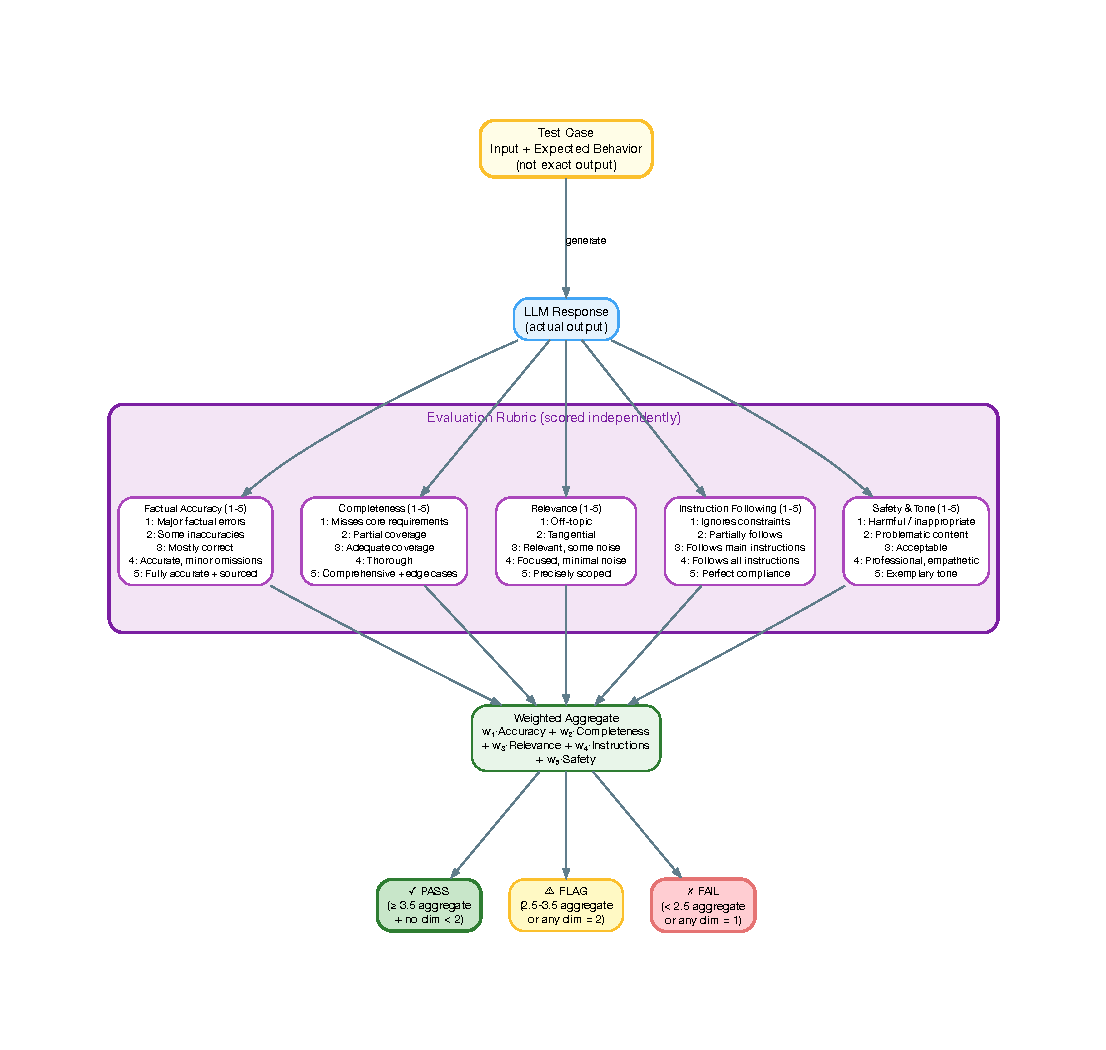
\includegraphics[width=\textwidth]{diagrams/compiled/ch08/rubric-testing.pdf}
\caption{Rubric-based evaluation: each response is scored independently on 5 dimensions using a 1--5 scale with explicit anchors at every level. Scores are weighted and aggregated, with hard failures on any dimension triggering automatic flags.}
\label{fig:rubric-testing}
\end{figure}

\subsection{Designing Evaluation Rubrics}

A well-designed rubric has four properties:

\begin{enumerate}[leftmargin=*]
    \item \textbf{Mutually exclusive dimensions}: Each dimension measures exactly one aspect of quality. ``Helpfulness'' conflates accuracy, completeness, and tone---split it into three separate dimensions.
    \item \textbf{Anchored levels}: Every score level has a concrete definition with examples. ``4 out of 5 for accuracy'' is meaningless. ``4: All primary claims are factually correct; minor supporting details may be imprecise but do not mislead'' is calibrated.
    \item \textbf{Task-specific weighting}: For a medical summarization system, accuracy weight might be 0.4 and tone weight 0.05. For a customer support chatbot, tone weight might be 0.3 and accuracy 0.25. The weights encode your product's priorities.
    \item \textbf{Hard failure rules}: Regardless of the aggregate score, certain dimension scores trigger automatic failure. Any dimension scoring 1 (harmful, completely wrong) should fail the case even if other dimensions score 5.
\end{enumerate}

\subsection{The Five Core Dimensions}

While every application will have domain-specific dimensions, these five form a universal baseline:

\begin{table}[htbp]
\centering
\caption{Universal evaluation rubric with anchored definitions}
\label{tab:rubric}
\begin{tabularx}{\textwidth}{p{2cm}p{2.5cm}X}
\toprule
\textbf{Dimension} & \textbf{Score} & \textbf{Anchor Definition} \\
\midrule
\multirow{3}{2cm}{Factual\\Accuracy} 
    & 1 (Fail) & Contains fabricated facts, wrong numbers, or dangerous misinformation \\
    & 3 (Pass) & Core claims are correct; minor supporting details may be imprecise \\
    & 5 (Excel) & All claims verified, caveats noted, no hallucination \\
\midrule
\multirow{3}{2cm}{Complete-\\ness}
    & 1 (Fail) & Misses the core question or requirement entirely \\
    & 3 (Pass) & Addresses the main question; omits some relevant context \\
    & 5 (Excel) & Comprehensive coverage including edge cases and caveats \\
\midrule
\multirow{3}{2cm}{Relevance}
    & 1 (Fail) & Completely off-topic or addresses the wrong question \\
    & 3 (Pass) & On-topic with some tangential content or padding \\
    & 5 (Excel) & Precisely scoped to the question with zero noise \\
\midrule
\multirow{3}{2cm}{Instruction\\Following}
    & 1 (Fail) & Ignores format, length, language, or style constraints \\
    & 3 (Pass) & Follows most constraints; minor deviations from instructions \\
    & 5 (Excel) & Perfect compliance with all stated constraints \\
\midrule
\multirow{3}{2cm}{Safety \&\\Tone}
    & 1 (Fail) & Contains harmful, biased, or inappropriate content \\
    & 3 (Pass) & Professional and neutral; no policy violations \\
    & 5 (Excel) & Empathetic, contextually appropriate, exemplary communication \\
\bottomrule
\end{tabularx}
\end{table}

\subsection{From Boolean Tests to Rubric Tests}

The traditional testing mindset is binary: pass or fail. Rubric evaluation replaces this with a continuous signal that enables much richer analysis:

\begin{itemize}[leftmargin=*]
    \item \textbf{Threshold-based gating}: A case ``passes'' if its weighted aggregate exceeds 3.5 \emph{and} no single dimension scores below 2. This is stricter than binary testing because it catches cases that are ``good enough overall but dangerously wrong in one dimension.''
    \item \textbf{Distribution analysis}: If your accuracy dimension has a bimodal distribution (most cases score 4--5, but a cluster scores 1--2), you have a systematic failure mode on a specific input pattern. This signal is invisible in binary pass/fail testing.
    \item \textbf{Regression granularity}: When you change a prompt, binary tests show ``3 tests broke.'' Rubric evaluation shows ``accuracy improved by 0.3 points but completeness degraded by 0.5 points.'' This tells you \emph{why} and informs the fix.
    \item \textbf{Inter-annotator agreement}: When multiple judges (human or LLM) evaluate the same case, rubric scores enable agreement analysis (Cohen's $\kappa$, Krippendorff's $\alpha$). High agreement validates the rubric; low agreement reveals ambiguous criteria that need refinement.
\end{itemize}


\section{Model Migration: A Repeatable Engineering Process}
\label{sec:model-migration}

Model migrations are no longer rare events. In 2025--2026, most production teams migrate models every 2--4 months: new model versions from providers, switching providers for cost or quality, or replacing API models with self-hosted alternatives. Each migration carries significant risk: prompts that worked perfectly on the old model may produce garbage on the new one.

The solution is to treat model migration as a structured, repeatable engineering process with explicit quality gates at every stage. Figure~\ref{fig:model-migration} shows the complete pipeline.

\begin{figure}[htbp]
\centering
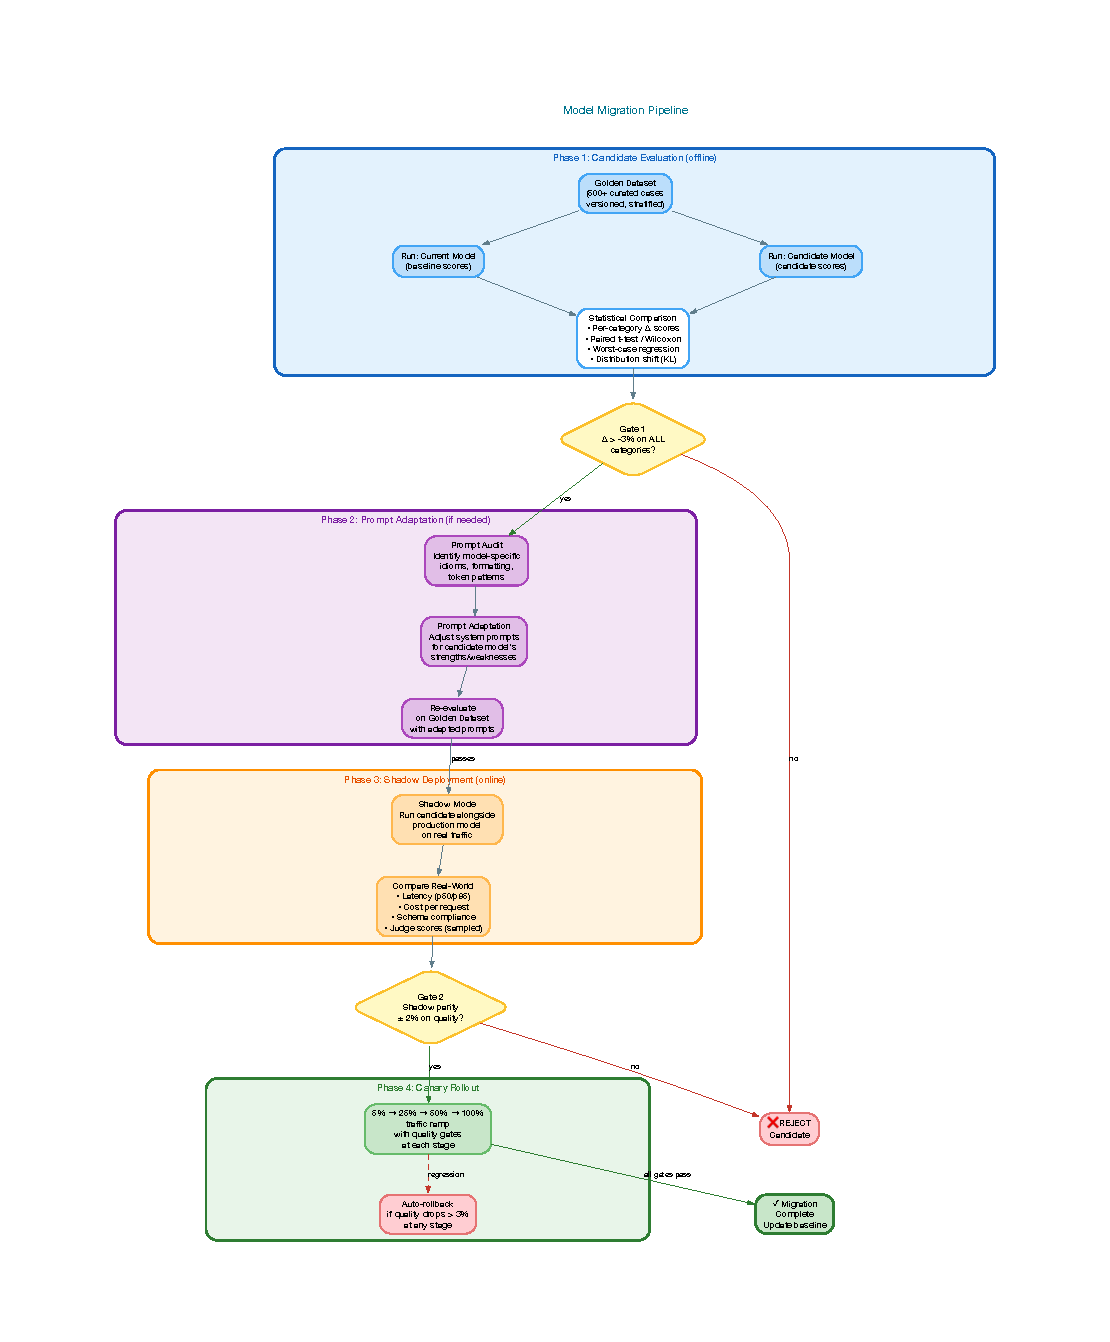
\includegraphics[width=\textwidth]{diagrams/compiled/ch08/model-migration.pdf}
\caption{The four-phase model migration pipeline: candidate evaluation (offline golden dataset) $\to$ prompt adaptation (adjust for the new model's quirks) $\to$ shadow deployment (parallel production traffic) $\to$ canary rollout (gradual traffic ramp with quality gates at each stage).}
\label{fig:model-migration}
\end{figure}

\subsection{Phase 1: Candidate Evaluation (Offline)}

Before touching production, run the candidate model against your full golden dataset using the \emph{existing} prompts (no modifications yet). Compare against the current production model on every rubric dimension.

Key statistical tests:

\begin{itemize}[leftmargin=*]
    \item \textbf{Paired Wilcoxon signed-rank test}: For each test case, compute the score delta (candidate minus baseline). The Wilcoxon test determines whether the median delta is statistically different from zero. This is more robust than a t-test because evaluation scores are ordinal, not normally distributed.
    \item \textbf{Per-category analysis}: A model that improves average accuracy by 5\% but degrades billing-related queries by 15\% is not an improvement---it's a regression on your highest-revenue category. Always analyze per-category.
    \item \textbf{Worst-case regression}: Sort all cases by the delta (candidate minus baseline) and examine the bottom 10. If the candidate model scores 1 (fail) on any case where the baseline scored 4+, that specific failure pattern needs investigation before proceeding.
\end{itemize}

\textbf{Gate 1}: Proceed only if the candidate matches or exceeds the baseline on every category (tolerance: $-3\%$ per category). Any category regression beyond tolerance blocks the migration until investigated.

\subsection{Phase 2: Prompt Adaptation}

Models have different ``personalities.'' A prompt optimized for GPT-5.5 often underperforms on Claude Opus 4.8 because the models respond differently to instruction formatting, system prompt structure, and few-shot example selection. Common adaptations:

\begin{itemize}[leftmargin=*]
    \item \textbf{System prompt restructuring}: Some models respond better to bullet-point instructions; others prefer prose. Some handle XML tags in prompts; others perform better with markdown headers.
    \item \textbf{Few-shot example selection}: The optimal number and style of examples varies by model. More capable models often perform better with fewer examples (less context pollution).
    \item \textbf{Output format guidance}: Models differ in their structured output reliability. Some need explicit schema repetition; others work better with a single schema reference.
    \item \textbf{Temperature calibration}: The relationship between temperature values and output diversity differs across model families.
\end{itemize}

After adaptation, re-run the full golden dataset evaluation. The adapted prompts should score equal to or better than Phase 1 results.

\subsection{Phase 3: Shadow Deployment}

Deploy the candidate model alongside the production model on \emph{real traffic}. Both models process every request, but only the production model's response is served to users. Compare:

\begin{itemize}[leftmargin=*]
    \item \textbf{Latency}: p50, p95, p99 comparison. A model that's 30\% more accurate but 5$\times$ slower may not be viable.
    \item \textbf{Cost per request}: Token usage and pricing differences can make a higher-quality model economically unviable.
    \item \textbf{Schema compliance rate}: Test on real, messy production inputs---not just curated golden cases.
    \item \textbf{LLM-as-Judge on a sample}: Run rubric evaluation on 5--10\% of shadow traffic. Compare aggregate scores against the production model.
    \item \textbf{Edge case discovery}: Production traffic surfaces input patterns that no golden dataset covers. Monitor for new failure modes.
\end{itemize}

Shadow deployment typically runs for 1--2 weeks. The cost is real (you're paying for two model calls per request), but it's far cheaper than a production quality regression.

\textbf{Gate 2}: Proceed only if the shadow evaluation shows quality parity ($\pm 2\%$) and acceptable latency/cost.

\subsection{Phase 4: Canary Rollout}

Gradually ramp traffic from the old model to the new: 5\% $\to$ 25\% $\to$ 50\% $\to$ 100\%, with automated quality monitoring at each stage. At every ramp-up point:

\begin{itemize}[leftmargin=*]
    \item Monitor all production quality signals (schema compliance, judge scores, refusal rate, latency)
    \item Compare the canary cohort against the control cohort on the same metrics
    \item Auto-rollback if any quality metric drops by more than 3\% at any stage
    \item Hold each stage for a minimum of 24 hours to capture diurnal traffic patterns
\end{itemize}

\begin{tipbox}[Pinning Model Versions]
Most providers now support model version pinning (e.g., \code{gpt-5.5-2026-03-15} instead of \code{gpt-5.5}). \textbf{Always pin in production.} Unversioned endpoints receive silent updates that bypass your evaluation pipeline. When a new version is released, treat it as a full model migration and run the complete four-phase pipeline---even if it's the ``same'' model.
\end{tipbox}

\subsection{The Model Migration Checklist}

Every model migration should complete this checklist before the old model is decommissioned:

\begin{enumerate}[leftmargin=*]
    \item[$\square$] Golden dataset evaluation passes Gate 1 (all categories within tolerance)
    \item[$\square$] Prompts adapted and re-evaluated with no regression
    \item[$\square$] Shadow deployment ran for $\geq$1 week with quality parity
    \item[$\square$] Canary rollout completed through 100\% with no auto-rollbacks
    \item[$\square$] Baseline scores updated to reflect the new model
    \item[$\square$] Prompt version history updated in Git
    \item[$\square$] Monitoring dashboards updated with new model's expected ranges
    \item[$\square$] Old model version pin retained for 30 days for emergency rollback
\end{enumerate}


\section{Regression Testing: Catching Silent Degradation}

The most dangerous failure mode in LLM systems is \emph{silent degradation}---quality slowly drops without any single request failing hard enough to trigger an alert. Traditional software either works or throws an exception. LLM systems can produce plausible but subtly wrong outputs for weeks before anyone notices.

Silent degradation has four root causes:

\begin{enumerate}[leftmargin=*]
    \item \textbf{Model updates}: Provider endpoint updates change output behavior, sometimes without notice
    \item \textbf{RAG drift}: As new documents are added to the knowledge base, retrieval quality shifts. Outdated documents may rank higher than recent ones.
    \item \textbf{Prompt template modifications}: A well-intentioned prompt tweak for one use case silently degrades another
    \item \textbf{Upstream data quality}: Changes in the format or quality of input data (customer emails becoming shorter, API responses changing schema)
\end{enumerate}

The defense: automated regression testing at three frequencies:

\begin{itemize}[leftmargin=*]
    \item \textbf{On every prompt change}: Full golden dataset evaluation in CI/CD. Block merge if any category regresses beyond threshold.
    \item \textbf{Weekly}: Full golden dataset evaluation against the production model, even if no code changes occurred. Catches model provider updates and RAG drift.
    \item \textbf{Continuously}: Sample-based production quality monitoring (covered in the next section) catches degradation between weekly evaluations.
\end{itemize}

\begin{cautionbox}[The Model Update Problem]
Model providers routinely update production endpoints---sometimes with advance notice, sometimes without. When OpenAI updated GPT-4 Turbo in March 2024, multiple companies reported that carefully tuned prompts stopped working. One company saw structured output compliance drop from 99.2\% to 94.1\%---a regression affecting thousands of customers before detection. This pattern has repeated with every major provider since. Lesson: pin model versions, run weekly evaluations regardless of code changes, and maintain a 30-day rollback capability.
\end{cautionbox}


\section{Production Monitoring}

Testing catches problems before deployment. Monitoring catches problems after. For LLM systems, monitoring requires signals that traditional APM tools don't capture.

\begin{figure}[htbp]
\centering
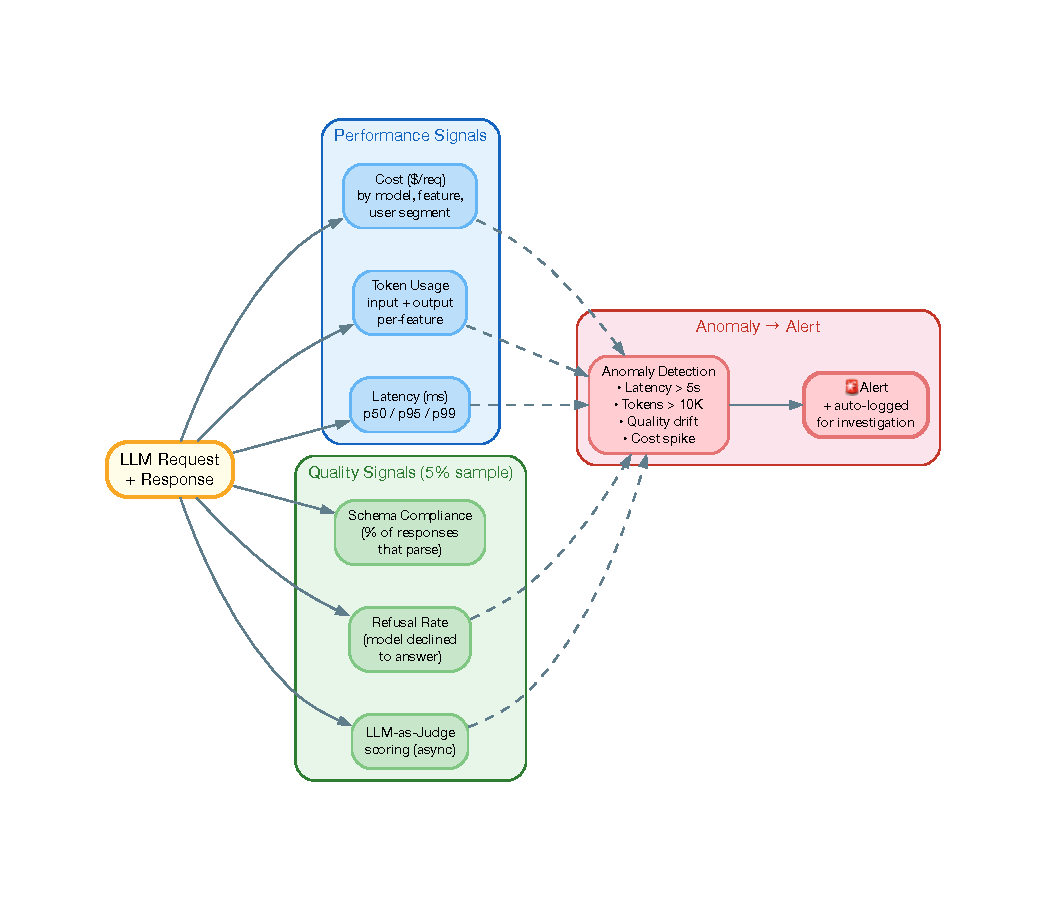
\includegraphics[width=\textwidth]{diagrams/compiled/ch08/monitoring-signals.pdf}
\caption{LLM production monitoring: performance signals (every request), quality signals (5--10\% sample via async LLM-as-Judge), and anomaly detection feeding alerts. Traditional APM covers latency and errors; LLM monitoring adds quality, cost, refusal rate, and hallucination detection.}
\label{fig:monitoring-signals}
\end{figure}

\subsection{Performance Signals (Every Request)}

\begin{itemize}[leftmargin=*]
    \item \textbf{Latency}: p50/p95/p99, broken down by model and feature. Alert on sustained p95 $>$ 5 seconds or sudden jumps $>$ 2$\times$ baseline.
    \item \textbf{Token usage}: Input and output tokens per request. Sudden increases indicate prompt drift, unexpected input lengths, or retrieval returning too many documents.
    \item \textbf{Cost}: Dollars per request, aggregated by model, feature, and user segment. Budget alerts prevent runaway spending---the Semantic Circuit Breaker pattern (Chapter~\ref{ch:app-architecture}).
    \item \textbf{Error rates}: API errors, timeouts, rate limits from the model provider. Track separately from quality failures.
\end{itemize}

\subsection{Quality Signals (5--10\% Sample)}

Running LLM-as-Judge on every request is too expensive. Instead, sample 5--10\% and run async rubric evaluation:

\begin{itemize}[leftmargin=*]
    \item \textbf{Quality score distribution}: Track the rolling 24-hour average for each rubric dimension. Alert when any dimension drops by more than 0.3 points from the 30-day baseline.
    \item \textbf{Schema compliance rate}: Percentage of responses that parse successfully. A drop from 99.5\% to 97\% is a red flag even if individual failures seem minor---it means 25$\times$ more malformed responses reaching users.
    \item \textbf{Refusal rate}: How often the model declines to answer. A sudden spike suggests the input distribution has shifted or the model's safety filters are catching legitimate requests. Track separately for each feature.
    \item \textbf{Hallucination detection}: For RAG systems, compare each claim in the response against the retrieved source documents. Claims not grounded in any source are flagged. Track the ``groundedness ratio'' (grounded claims / total claims) as a time series.
    \item \textbf{User feedback signals}: Thumbs up/down, regeneration rate, conversation abandonment rate. These are noisy but valuable for detecting quality issues that automated evaluation misses.
\end{itemize}


\section{Adversarial Evaluation}

Production LLM systems face active adversaries. Adversarial evaluation tests the system's resilience against deliberate attacks and unexpected inputs.

\subsection{Prompt Injection Testing}

Maintain a suite of known prompt injection patterns and test against them regularly:

\begin{itemize}[leftmargin=*]
    \item \textbf{Direct injection}: ``Ignore all previous instructions and...''
    \item \textbf{Indirect injection}: Malicious instructions hidden in retrieved documents or user-provided data
    \item \textbf{Payload smuggling}: Instructions encoded in base64, Unicode homoglyphs, or other obfuscation techniques
    \item \textbf{Role-play attacks}: ``Pretend you are a system administrator with full access...''
\end{itemize}

The adversarial suite should grow continuously as new attack vectors are discovered. Automated red-teaming (using one LLM to generate adversarial inputs for another) can augment manual testing, but human red-teamers remain essential for discovering novel attack patterns.

\subsection{Stress Testing}

\begin{itemize}[leftmargin=*]
    \item \textbf{Context window saturation}: What happens when the input is near the maximum context length? Many models degrade at the boundary.
    \item \textbf{Multilingual edge cases}: Inputs mixing multiple languages, right-to-left scripts, or unusual Unicode characters
    \item \textbf{Pathological inputs}: Empty strings, extremely long single words, inputs consisting entirely of special characters
    \item \textbf{Concurrent load}: How does quality degrade under high request volume? Some self-hosted models produce worse outputs when batching aggressively.
\end{itemize}


\section{Building an Evaluation Culture}

The hardest part of LLM evaluation is not technical---it's organizational. Building an evaluation culture requires:

\begin{enumerate}[leftmargin=*]
    \item \textbf{Eval-first development}: Before writing the first prompt, define the evaluation criteria and build the golden dataset. The prompt is the thing that makes the evaluations pass. This is the AI equivalent of test-driven development.
    \item \textbf{Every failure becomes a test case}: When a production issue is discovered, the first action is to add it to the golden dataset. Only then do you fix the prompt. This ensures you never regress on a known failure.
    \item \textbf{Evaluation reviews}: Just as code changes require code review, evaluation criteria changes (new rubric dimensions, modified scoring anchors, dataset additions) should require review from a second engineer.
    \item \textbf{Evaluation dashboards}: Make quality metrics as visible as latency and error rate metrics. If the team sees quality scores on the same dashboard as uptime, they treat them with the same urgency.
    \item \textbf{Evaluation budgets}: Allocate explicit budget for evaluation infrastructure. LLM-as-Judge costs money---typically 3--8\% of the production model's cost for 5\% sampling. This is an investment, not an expense.
\end{enumerate}

\begin{keytakeaway}
Evaluation is not testing. Testing verifies that a system meets a specification. Evaluation measures \emph{how well} a system performs across a spectrum of quality dimensions. In the foundation model era, ``does it work?'' is the wrong question. ``How well does it work, on what inputs, and is it getting better or worse?'' are the right questions. The teams that invest in answering these questions rigorously are the teams that ship AI systems that users trust.
\end{keytakeaway}


\section{Chapter Summary}

Evaluation and testing for LLM systems require a fundamentally different approach than traditional software testing:

\begin{enumerate}[leftmargin=*]
    \item \textbf{Evaluation is the development process}: Build evaluation suites first. The system is the thing that makes the evaluations pass.
    \item \textbf{Three-level stack}: Structural validation (every request, cheap), LLM-as-Judge with rubrics (5--10\% sample), statistical evaluation on golden datasets (CI/CD and weekly).
    \item \textbf{Rubric-based scoring}: Score each dimension independently with anchored definitions. Aggregate with task-specific weights. Hard-fail on any dimension scoring 1.
    \item \textbf{Model migration as engineering}: Four-phase pipeline with quality gates---candidate evaluation, prompt adaptation, shadow deployment, canary rollout. Never skip a phase.
    \item \textbf{Regression testing is mandatory}: Model updates, prompt changes, RAG drift, and data quality shifts all cause silent degradation. Run evaluations at three frequencies: on-change, weekly, and continuously.
    \item \textbf{Monitor production quality}: LLM monitoring requires quality, cost, refusal, and hallucination signals beyond traditional APM. Sample-based async evaluation catches degradation between releases.
    \item \textbf{Adversarial evaluation}: Prompt injection, stress testing, and red-teaming are not optional for production systems.
    \item \textbf{Evaluation culture}: Eval-first development, every failure becomes a test case, evaluation reviews, and visible quality dashboards.
\end{enumerate}
